\thispagestyle{plain}
\begin{center}
\Large\textbf{Growth of interface cracks on consecutive fibers: on the same or on the opposite sides?}\\
\vspace{10mm}
\normalsize Luca Di Stasio$^{1,2}$, Janis Varna$^{1}$ and Zoubir Ayadi$^{2}$\\
\vspace{5mm}
\normalsize $^{1}$Lule\aa\ University of Technology, University Campus, SE-97187 Lule\aa, Sweden\\
\normalsize $^{2}$Universit\'e de Lorraine, EEIGM, IJL, 6 Rue Bastien Lepage, F-54010 Nancy, France\\
\vspace{15mm}
\textbf{Abstract}\\
\end{center}

The growth of fiber/matrix interface cracks (debonds) located on consecutive fibers along the through-the-thickness (vertical) direction is studied in glass fiber-epoxy UD composites. Two different families of Representative Volume Elements (RVEs) are developed: the first implements the classic condition of coupling of the vertical displacements to model a unit cell repeating symmetrically along the vertical direction; the second uses a novel set of boundary conditions, proposed here by the authors, to represent a unit cell repeating anti-symmetrically along the vertical direction. The model is analyzed in the context of Linear Elastic Fracture Mechanics (LEFM) and the Mode I and Mode II Energy Release Rate are evaluated to investigate crack growth. The calculation is performed using the Virtual Crack Closure Technique (VCCT) in the framework of the Finite Element Method (FEM). It is found that Mode I dominated propagation is favored when debonds are located on the same sides of their respective fibers; while for larger Mode II-dominated debonds, Mode II ERR is higher when they lie on the opposite sides. No effect is present when at least two fully bonded fibers are located between the partially debonded ones.

\vspace{5mm}

\textbf{Keywords:} Polymer Matrix Composite (PMC), Transverse cracking, Debonding, Debond Interaction


%%%%%%%%%%%%%%%%%%%%%%%%%%%%%%%%%%%%%%%%%%%%%%%%%%%%%%%%%%%%%%%%%%%
% 1. INTRODUCTION
%%%%%%%%%%%%%%%%%%%%%%%%%%%%%%%%%%%%%%%%%%%%%%%%%%%%%%%%%%%%%%%%%%%

\section{Introduction}

Organized and completed over the last three decades, the three World Wide Failure Exercises (WWFEs)~\cite{Hinton2004,Hinton2012,Kaddour2013a} represent one of the most comprehensive attempts to date to evaluate the maturity of failure criteria and predictive theories of damage of Fiber-Reinforced Polymer Composites (FRPC). The third and last one (WWFE-III) aims at providing a benchmark for models of sub-critical damage, namely matrix cracking, delamination and fiber failure, by comparing the independent predictions of 12 different approaches (each one from a different individual, group or institution) over 13 test cases~\cite{Kaddour2013a}. The comparison of predictions by the different theories shows a wide scatter of results, symptomatic of the immaturity of the field~\cite{Kaddour2013b}. Furthermore, it uncovers the existence of gaps in the knowledge shared by all models. Among these, a clear understanding is still elusive regarding the mechanisms of initiation of an individual transverse crack.\\
Onset of transverse cracks is determined at the microscopic level by initiation and propagation of fiber-matrix interface cracks~\cite{Bailey1981,Bailey1979}, or debonds. Debonds first grow along the arc direction of the fiber; at a certain critical size they kink out of the interface and lead to the onset of matrix micro-cracks; micro-cracks coalesce together forming a through-the-thickness crack~\cite{Zhang1997}; this crack finally propagates along the fiber direction, i.e. “tunneling” across the width of the laminate, and creating a transverse crack. Thus, understanding the mechanism of debond growth and predicting debond critical arc size (at which kinking starts) represent an important step in the development of precise predictive models of transverse cracking.

\begin{figure}[!htb]
\centering
  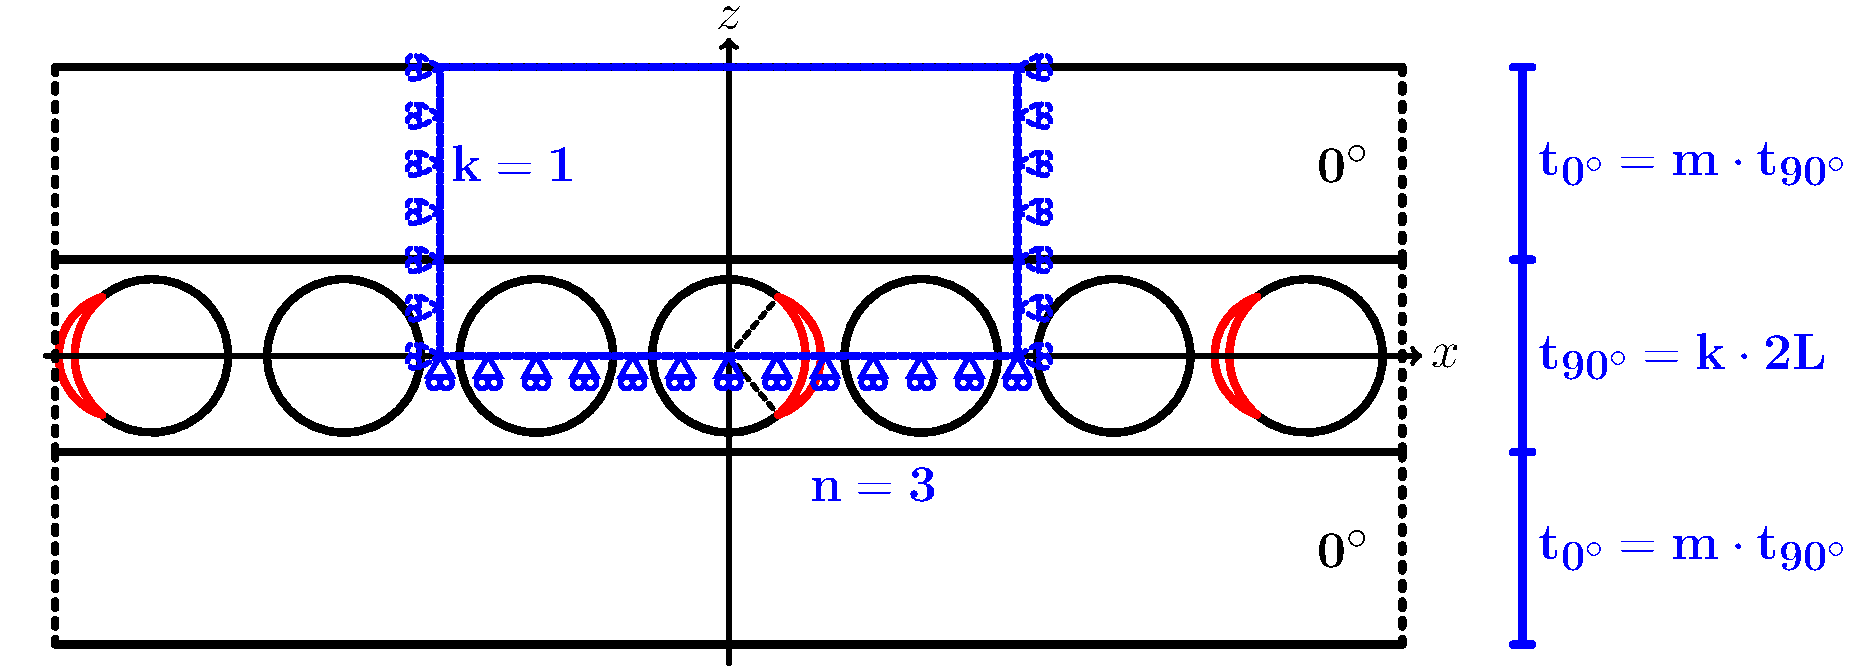
\includegraphics[height=0.225\textheight]{paperD/thinPly.pdf}
\caption{Debonds in the $90^{\circ}$ layer of a $\left[0^{\circ}/90^{\circ}\right]_{S}$ laminate after being subjected to tensile strain in the horizontal direction.}\label{paperD:fig:debonds-microscope}
\end{figure}

Initial attempts to analyze the mechanics of debonding were based on the linear elastic solution of a single partially debonded fiber in an infinite matrix with an applied tensile stress at infinity, evaluated analytically by using complex potentials ~\cite{England1966,Perlman1967,Toya1974}. It was found that stress and displacement fields have an oscillating singularity at the crack tip, which prevents the use of Stress Intensity Factors (SIFs) as they are not defined at the debond tip. Similarly, Mode I and Mode II Energy Release Rate (ERR) do not converge and mode-based partition of the ERR is not possible. However, the ERR can be interpreted as the work needed to open the crack by an infinitesimal amount da or equivalently, in the case of Linear Elastic Fracture Mechanics, to close the crack by the same infinitesimal amount $da$. By considering a small but finite crack increase $\Delta a$ instead of the infinitesimal increase $da$, the lack of convergence due to the oscillatory singularity can be circumvented and an approximation of Mode I and Mode II ERR can be provided. The recurse to this strategy makes the problem suitable for a resolution technique based on domain discretization such as the Finite Element Method (FEM) or the Boundary Element Method (BEM). In subsequent works~\cite{Paris1996,Varna1997a}, it was shown that Toya’s analytical solution~\cite{Toya1974} implies a non-physical interpenetration zone in the crack tip neighborhood. This led to the introduction of a no-interpenetration contact interaction which, solved with the Boundary Element Method (BEM), showed the existence of a contact zone (a finite size region in which crack faces are in contact) for debonds larger than a critical value~\cite{Varna1997a}. In ~\cite{Garcia2015}, the authors compared the one-debond with respect to the two-symmetric-debonds configuration and found that the former is energetically the most favorable to crack growth. The effect of several load combinations on ERR of a single partially debonded fiber in an effectively infinite matrix was later studied~\cite{Correa2007,Correa2013,Correa2014}, as well as the effect of a neighboring fully bonded fiber~\cite{Sandino2016,Zhuang2018}. Researchers in~\cite{Varna2017} studied the effect on debond ERR of the presence of a second partially debonded fiber, with the two debonds placed facing each other (i.e. no fiber in between).\\
Microscopic observations of debond growth, such as the one reported in Fig.~\ref{paperD:fig:debonds-microscope}, show debonds developed on the same as well as the opposite sides of consecutive fibers on average aligned along the vertical, i.e. through-the thickness, direction. It is thus interesting to investigate the effect on debond ERR of the position of the next debond on the neighboring partially debonded fiber along the vertical direction. To this end, we develop Representative Volume Elements (RVEs) which, by application of displacement-coupling boundary conditions along the right and left sides, are repeating in a mirror-like fashion horizontally. The use of coupling conditions on the vertical displacement along the upper boundary models the presence of another partially debonded fiber with a debond of equal size and on the same side. In order to model the case of a fiber with a debond of equal size but appearing on the opposite side, we propose a set of anti-symmetric coupling conditions that are applied to the upper boundary. Details regarding coupling conditions, RVEs and Finite Element (FE) discretization are presented in Sec. \ref{paperD:sec:RVEs} and Sec. 3, while results are presented and discussed in Sec. 4.

%%%%%%%%%%%%%%%%%%%%%%%%%%%%%%%%%%%%%%%%%%%%%%%%%%%%%%%%%%%%%%%%%%%
% 2. RVE MODELS AND FE DISCRETIZATION
%%%%%%%%%%%%%%%%%%%%%%%%%%%%%%%%%%%%%%%%%%%%%%%%%%%%%%%%%%%%%%%%%%%

\section{Representative Volume Elements (RVEs)}\label{paperD:sec:RVEs}



%%%%%%%%%%%%%%%%%%%%%%%%%%%%%%%%%%%%%%%%%%%%%%%%%%%%%%%%%%%%%%%%%%%
% 3. RESULTS AND DISCUSSION
%%%%%%%%%%%%%%%%%%%%%%%%%%%%%%%%%%%%%%%%%%%%%%%%%%%%%%%%%%%%%%%%%%%

\section{Results \& Discussion}

\subsection{Effect of the proximity of the $0^{\circ}/90^{\circ}$ interface and of the thickness of the $0^{\circ}$ layer on debond ERR for highly interactive debonds}\label{paperC:subsec:thickness}

We first focus our attention on the model $1\times 1-m\cdot t_{90^{\circ}}$, which represents a particular case of the family $n\times 1-m\cdot t_{90^{\circ}}$. It corresponds to a cross-ply laminate in which the central $90^{\circ}$ ply is constituted by only one fiber row, in which each fiber possesses a debond appearing on alternating sides. The model thus represents an extreme idealization, in the sense that: first, the central $90^{\circ}$ layer is the thinniest that can be conceived, which allows us to investigate the direct effect of the proximity of the $0^{\circ}/90^{\circ}$ interface on debond ERR; second, a very particular damage state is present for which every fiber is partially debonded from the sorrounding matrix, corresponding to the most severe damage state that can occur in the $90^{\circ}$ ply when considering debonds as the only mechanism of damage. We are thus focusing on the presence of the $0^{\circ}/90^{\circ}$ interface and on the thickness of the $0^{\circ}$ layer, by considering the ratio $m=\frac{t_{0^{\circ}}}{t_{90^{\circ}}}$ of ply thicknessess as a free parameter.\\

\begin{figure}[!htb]
\centering
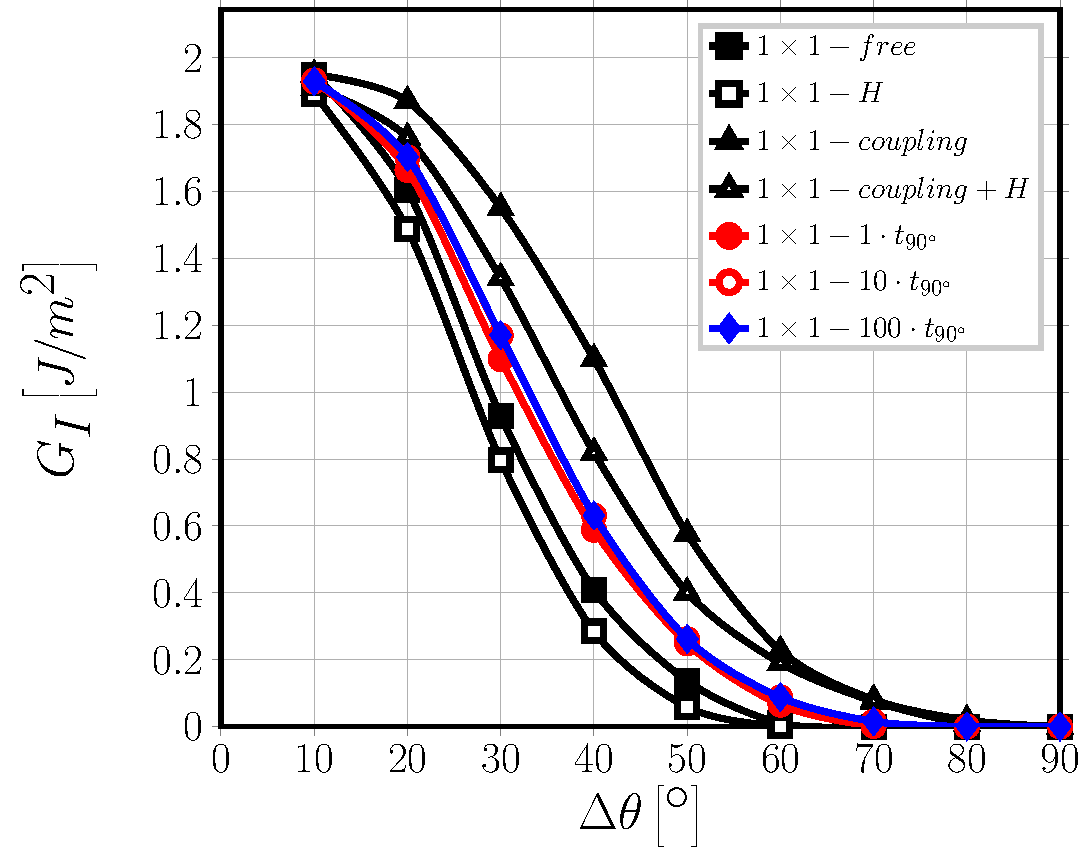
\includegraphics[height=0.375\textheight]{paperC/1x1-i-vf60-GI.pdf}
\caption{Effect of the proximity of the $0^{\circ}/90^{\circ}$ interface and of the thickness of the $0^{\circ}$ layer on Mode I ERR: models $1\times 1-free$, $1\times 1-H$, $1\times 1-coupling$, $1\times 1-coupling+H$ and $1\times 1-m\cdot t_{90^{\circ}}$. $V_{f}=60\%$, $\bar{\varepsilon}_{x}=1\%$.}\label{paperC:fig:thicknessGI}
\end{figure}

In Figures~\ref{paperC:fig:thicknessGI} and~\ref{paperC:fig:thicknessGII} it is possible to observe respectively the Mode I and Mode II ERR for models $1\times 1-m\cdot t_{90^{\circ}}$ with $m=1,10,100$. Mode I ERR is practically unaffected by the $0^{\circ}$ layer thickness, only a marginal increase $\leq1\%$ can be seen when $m$ is increased from $1$ to $10$. No further observable change is present when $m$ is increased to $100$. Moreover, the contact zone onset, which corresponds to the first value of $\Delta\theta$ such that $G_{I}=0$, is always equal to $70^{\circ}$ irrespective of the value of $m$. A more remarkable, albeit small, effect of the $0^{\circ}$ layer thickness can be observed for Mode II when $m$ is increased from $1$ to values $\geq10$. For open cracks, i.e. when no contact zone is present and thus $\Delta\theta$ is smaller than $70^{\circ}$, increasing the $0^{\circ}$ layer thickness causes a reduction of Mode II ERR; while for closed cracks, when a contact zone is present and $\Delta\theta>70^{\circ}$, the increase in thickness leads to an increase in ERR.\\

\begin{figure}[!htb]
\centering
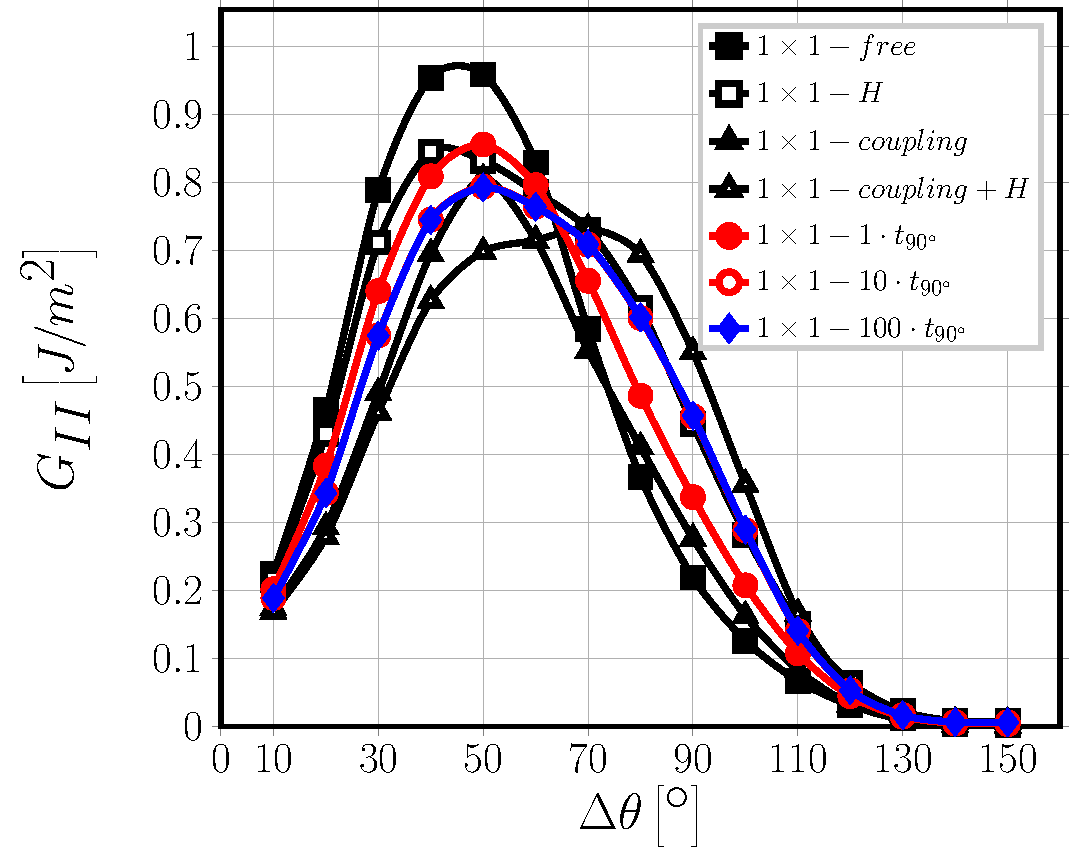
\includegraphics[height=0.375\textheight]{paperC/1x1-i-vf60-GII.pdf}
\caption{Effect of the proximity of the $0^{\circ}/90^{\circ}$ interface and of the thickness of the $0^{\circ}$ layer on Mode II ERR: models $1\times 1-free$, $1\times 1-H$, $1\times 1-coupling$, $1\times 1-coupling+H$ and $1\times 1-m\cdot t_{90^{\circ}}$. $V_{f}=60\%$, $\bar{\varepsilon}_{x}=1\%$.}\label{paperC:fig:thicknessGII}
\end{figure}

In order to understand the interaction mechanism between the $0^{\circ}/90^{\circ}$ interface and the debond, Mode I and Mode II ERR are reported respectively in Figures~\ref{paperC:fig:thicknessGI} and~\ref{paperC:fig:thicknessGII} for models $1\times 1-free$, $1\times 1-H$, $1\times 1-coupling$ and $1\times 1-coupling+H$. These RUCs all present equivalent boundary conditions and it is here useful to recall their characteristics: in model $1\times 1-free$ the upper bounday is left free; coupling conditions on the vertical displacements $u_{z}$ are applied to the upper boundary in model $1\times 1-coupling$ (coupling condition); in model $1\times 1-H$ a linearly distributed horizontal displacement $u_{x}$ is applied to the upper boundary (H-condition); in model $1\times 1-coupling+H$ coupling conditions on the vertical displacements $u_{z}$ and a linearly distributed horizontal displacement $u_{x}$ are imposed together on the upper boundary. Given that the presence of a $0^{\circ}$ layer provides two constraints: first, it tends to keep the $90^{\circ}$ layer boundary straight; second, it forces a more homogeneous horizontal displacement at the $90^{\circ}$ layer boundary; the equivalent boundary conditions of $1\times 1-coupling$, $1\times 1-H$ and $1\times 1-coupling+H$ represent an extreme case respectively of the first constraint ($1\times 1-coupling$), the second constraint ($1\times 1-H$) and the two together ($1\times 1-coupling+H$). The case $1\times 1-free$ constitutes instead the base case (absence of $0^{\circ}$ layer), on which comparisons are built.\\
Observing Figure~\ref{paperC:fig:thicknessGI}, it is possible to notice that the values of $G_{I}$ for the $1\times 1-free$ and the $1\times 1-coupling$ models represent respectively a lower and an upper bound for the $1\times 1-m\cdot t_{90^{\circ}}$ RVEs: this is true with respect to the value of $G_{I}$ as well as of contact zone onset ($60^{\circ}$ for  $1\times 1-free$, $70^{\circ}$ for $1\times 1-m\cdot t_{90^{\circ}}$, $80^{\circ}$ for $1\times 1-coupling$). When the H-condition is added to the $1\times 1-free$ and the $1\times 1-coupling$ models, thus obtaining the $1\times 1-H$ and $1\times 1-coupling+H$ models, $G_{I}$ decreases while the value of $\Delta\theta$ at contact zone onset remains unchanged ($60^{\circ}$ for  $1\times 1-free$ and $1\times 1-H$, $80^{\circ}$ for $1\times 1-coupling$ and $1\times 1-coupling+H$). Moreover, it is possible to observe that the values of $G_{I}$ of $1\times 1-coupling+H$ are much closer to but always greater than those of $1\times 1-m\cdot t_{90^{\circ}}$ RVEs, thus constituting a more representative upper bound for the latter.\\
Analogous considerations are drawn with regard to Mode II (see Fig.~\ref{paperC:fig:thicknessGII}). For small debonds, $\Delta\theta\leq30^{\circ}$, no significant difference in $G_{II}$ can be seen between $1\times 1-free$ and $1\times 1-H$ and between $1\times 1-coupling$ and $1\times 1-coupling+H$ in this region. With respect to $1\times 1-m\cdot t_{90^{\circ}}$ RVEs, the first pair ($1\times 1-free$ and $1\times 1-H$) represents the lower bound while the second pair ($1\times 1-coupling$ and $1\times 1-coupling+H$) the upper bound. For $30^{\circ}<\Delta\theta\leq60^{\circ}$, $1\times 1-H$ and $1\times 1-coupling+H$ provide significantly lower values of $G_{II}$ than respectively $1\times 1-free$ and $1\times 1-coupling$. $G_{II}$ values of $1\times 1-H$ are very close to $1\times 1-1\cdot t_{90^{\circ}}$, even coincident for $\Delta\theta=60^{\circ}$. On the other hand, $G_{II}$ values of $1\times 1-coupling$ are very close to $1\times 1-m\cdot t_{90^{\circ}}$ with $m\geq10$ and even coincident for $\Delta\theta=50^{\circ}$. For $60^{\circ}<\Delta\theta\leq110^{\circ}$, the situation changes. $1\times 1-free$ and $1\times 1-coupling$ provides values of $G_{II}$ close to each other, even coincident for $\Delta\theta=70^{\circ}$. Values of $G_{II}$ of $1\times 1-H$ and $1\times 1-coupling+H$ are significantly larger than both $1\times 1-free$ and $1\times 1-coupling$. Furthermore, $G_{II}$ values of $1\times 1-H$ coincide with those of $1\times 1-m\cdot t_{90^{\circ}}$ with $m\geq10$. Mode II ERR of $1\times 1-1\cdot t_{90^{\circ}}$ is instead close, but not coincident, to that of $1\times 1-coupling$. For $\Delta\theta>110^{\circ}$, $G_{II}$ is the same for all models and reaches $0$ at a debond size of around $130^{\circ}$.\\
These results help to understand the effect of the $0^{\circ}/90^{\circ}$ interface on debond ERR. Two constraining mechanisms are present in the case of $0^{\circ}/90^{\circ}$ interface that are absent in the free surface case: first, the boundary of the $90^{\circ}$ layer remains straighter (effect modelled by the coupling condition in $1\times 1-coupling$); second, the $x$-strain on the $90^{\circ}$ layer boundary is more uniform (effect modelled by the H-condition in $1\times 1-H$).\\
%The presence of the stiff homogenized $0^{\circ}$ layer causes the matrix placed relatively far from the fiber (close to the interface) to contract less than it would do in the presence of a free surface due to its relatively high Poisson's ratio. In the free surface case, the contraction ($z$-strain) would be different at different positions along the $x$-axis as the $x$-strain is not uniform; in the presence of the $0^{\circ}/90^{\circ}$ interface, the $x$-strain is instead more homogenuous and, consequently, the $z$-strain as well.\\
For small debonds ($\Delta\theta<60^{\circ}-70^{\circ}$), the presence of the $0^{\circ}/90^{\circ}$ interface causes an increase of $G_{I}$ and a decrease of $G_{II}$ with respect to the free surface case. For Mode I, the fact that the $90^{\circ}$ layer boundary remains straight (coupling condition) forces the debond to open more than in the free case, thus increasing $G_{I}$. However, the uniformity of the $x$-strain on the $90^{\circ}$ layer boundary reduces the local (in the debond neighborhood) $x$-strain magnification and contains the increase in $G_{I}$. This corresponds in Figure~\ref{paperC:fig:thicknessGI} to the fact that Mode I ERR for $1\times1-m\cdot t_{90^{\circ}}$ is always higher than $1\times1-free$ but lower than $1\times1-coupling$, and it is best approximated by $1\times1-coupling+H$. For Mode II in the case of small debonds, the presence of the $0^{\circ}$ layer  keeps the $0^{\circ}/90^{\circ}$ interface straighter and reduces the vertical contraction of the matrix, which contributes for the most part to Mode II in this range, thus leading to a decrease of $G_{II}$. The small effect of $0^{\circ}$ layer thickness on Mode II (Fig.~\ref{paperC:fig:thicknessGII}) can be explained in terms of local bending stiffness: a thinner $0^{\circ}$ layer ($\frac{t_{0^{\circ}}}{t_{90^{\circ}}}=1$) does not keep the $90^{\circ}$ layer boundary as straight as thicker $0^{\circ}$ layers ($\frac{t_{0^{\circ}}}{t_{90^{\circ}}}\geq10$). In the case $\frac{t_{0^{\circ}}}{t_{90^{\circ}}}=1$, the $90^{\circ}$ layer boundary deforms in a way that is similar to the free surface case, but smaller in magnitude. This corresponds to the fact that for $\Delta\theta<60^{\circ}-70^{\circ}$, in Figure~\ref{paperC:fig:thicknessGII}: $1\times1-1\cdot t_{90^{\circ}}$ is best approximated by $1\times1-H$ (curved $90^{\circ}$ layer boundary but uniform $x$-strain at the $90^{\circ}$ layer boundary that disfavors $G_{II}$), $1\times1-m\cdot t_{90^{\circ}},m\geq10$ is best approximated by $1\times1-coupling$ (straight $90^{\circ}$ layer boundary).\\
For debonds larger than $70^{\circ}$, the presence of the $0^{\circ}/90^{\circ}$ interface causes an increase of $G_{II}$ with respect to the free surface case. The uniform $x$-strain distribution on the $90^{\circ}$ layer boundary determined by the presence of the $0^{\circ}$ layer causes, with respect to the free case, the matrix $x$-strain to be higher in the $x\sim0$ neighborhood and lower around $x\sim\pm L$, in order to keep the average $\varepsilon_{x}$ at $1\%$. Given that for large debonds Mode II ERR is determined mostly by the magnitude of the $x$-strain gap (between the matrix $x$-strain and the fiber $x$-strain), an increase of $G_{II}$ is thus observed in the presence of the $0^{\circ}/90^{\circ}$ interface. Again, the observed effect of the $0^{\circ}$ layer thickness on Mode II for $\Delta\theta>60^{\circ}-70^{\circ}$ (Fig.~\ref{paperC:fig:thicknessGII}) can be discussed in terms of local $0^{\circ}$ layer bending stiffness. In the free case, it is the curvature of the material around the fiber that causes the $x$-strain reduction and thus a lower $G_{II}$. Thicker $0^{\circ}$ layers ($\frac{t_{0^{\circ}}}{t_{90^{\circ}}}\geq10$) prevent this $90^{\circ}$ boundary deformation to a greater extent than the thinner $t_{0^{\circ}}=t_{90^{\circ}}$ case: the $x$-strain (and thus $G_{II}$) increase is greater for $\frac{t_{0^{\circ}}}{t_{90^{\circ}}}\geq10$ than $\frac{t_{0^{\circ}}}{t_{90^{\circ}}}=1$.

\subsection{Effect of the proximity of the $0^{\circ}/90^{\circ}$ interface and of the thickness of the $0^{\circ}$ layer on non-interactive debonds in a one-fiber row $90^{\circ}$ ply}\label{paperC:subsec:debonddebondinter}

We turn now our attention to models $n\times 1-m\cdot t_{90^{\circ}}$, which correspond to a cross-ply laminate in which the central $90^{\circ}$ ply is constituted by only one fiber row where multiple partially debonded fibers are present with $n-1$ fully bonded fibers between them and debonds appear on alternating sides of consecutive damaged fibers (see Figure~\ref{paperC:fig:laminateModelsA}). %This class of models allows to study the effect of the presence of the $0^{\circ}$ layer and of its thickness on non-interactive debonds.
As observed in a previous work~\cite{DiStasio2019}, the presence of fully bonded fibers between partially debonded ones in the loading direction has a strong effect on debond ERR and controls the interaction between debonds. When $n$ is increased, both Mode I and Mode II increase: the addition of stiffer elements, in the form of fully bonded fibers, increase the strain applied to the damaged unit and thus causes higher values of ERR. Looked from this perspective, i.e. moving from the most to the least severe state of damage, this effect is referred to as ``strain magnification''~\cite{DiStasio2019}. There seems to exist a characteristic distance, measured in terms of fully bonded fibers, above which a change in the number of undamaged fibers affects only marginally, or even not at all, debond ERR. This distance, generally $n\sim20$, marks the transition between a non-interactive solution ($n>20$) and an interactive one ($n<20$). The ``strain magnification'' effect thus represents the transition from the interactive to the non-interactive solution. If in Sec.~\ref{paperC:subsec:thickness} we studied the effect of the proximity of the $0^{\circ}/90^{\circ}$ interface and of the thickness of the $0^{\circ}$ layer on interactive debonds ($1\times 1-\dots$), we analyze in the present section the effect of the $0^{\circ}/90^{\circ}$ interface and of the $0^{\circ}$ layer thickness on non-interactive ones ($n\times 1-\dots\text{ with }n>20$).\\

\begin{figure}[!htb]
\centering
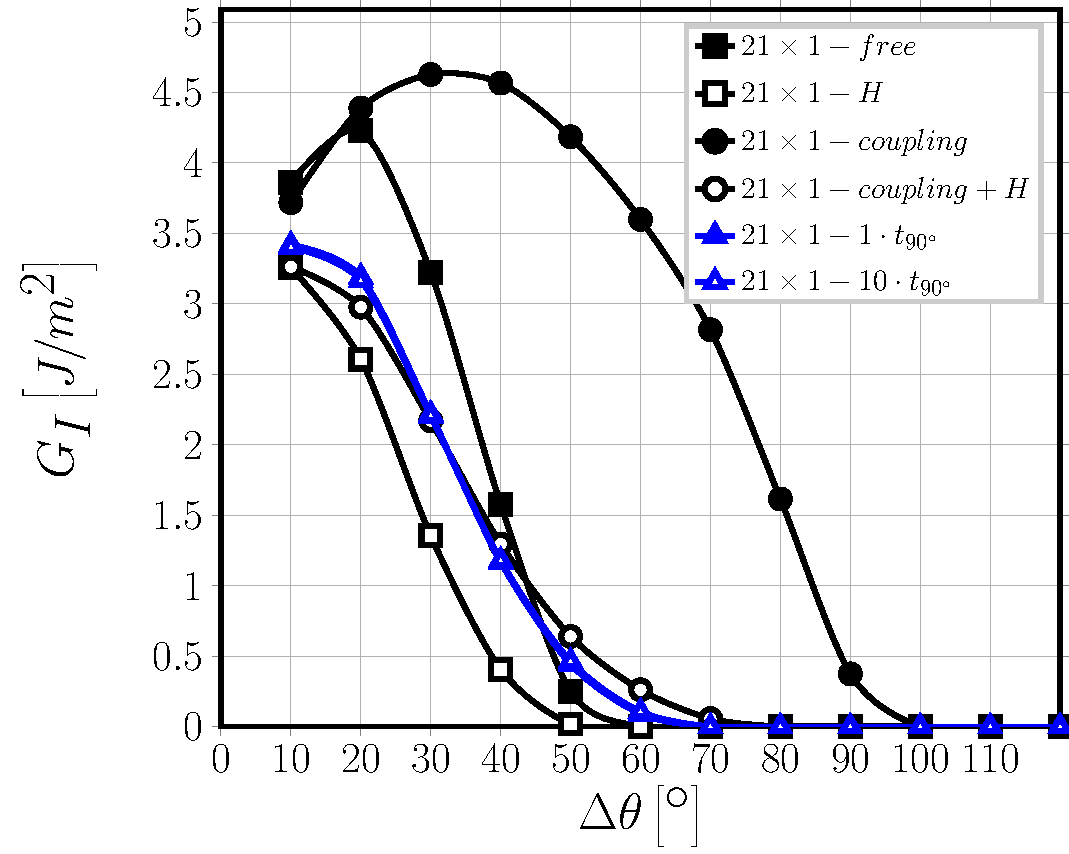
\includegraphics[height=0.375\textheight]{paperC/nx1-1-vf60-GI.pdf}
\caption{Effect of the presence of the $0^{\circ}$ layer on Mode I ERR of non-interactive debonds: models $21\times 1-free$, $21\times 1-H$, $21\times 1-coupling$, $21\times 1-coupling+H$, $21\times 1-1\cdot t_{90^{\circ}}$ and $21\times 1-10\cdot t_{90^{\circ}}$. $V_{f}=60\%$, $\bar{\varepsilon}_{x}=1\%$.}\label{paperC:fig:debonddebondGI}
\end{figure}

Comparing Fig.~\ref{paperC:fig:debonddebondGI} with Fig.~\ref{paperC:fig:thicknessGI} and Fig.~\ref{paperC:fig:debonddebondGII} with Fig.~\ref{paperC:fig:thicknessGII}, it is possible to observe how, as previously described, increasing the number of fully bonded fibers between consecutive debonds in the loading direction leads to an increase in Mode I and Mode II ERR. The peak $G_{I}$ increases from $1.93 \left[\frac{J}{m^{2}}\right]$ in $1\times 1-1\cdot t_{90^{\circ}}$ to $3.42 \left[\frac{J}{m^{2}}\right]$ in $21\times 1-1\cdot t_{90^{\circ}}$, while the peak $G_{II}$ from $0.86 \left[\frac{J}{m^{2}}\right]$ to $3.04 \left[\frac{J}{m^{2}}\right]$. The value of $\Delta\theta$ at contact zone onset remains however the same ($70^{\circ}$).\\
The effect of the $0^{\circ}$ layer thickness is instead non-existent: values of both $G_{I}$ and $G_{II}$ are coincident for $21\times 1-1\cdot t_{90^{\circ}}$ and $21\times 1-10\cdot t_{90^{\circ}}$.\\

\begin{figure}[!htb]
\centering
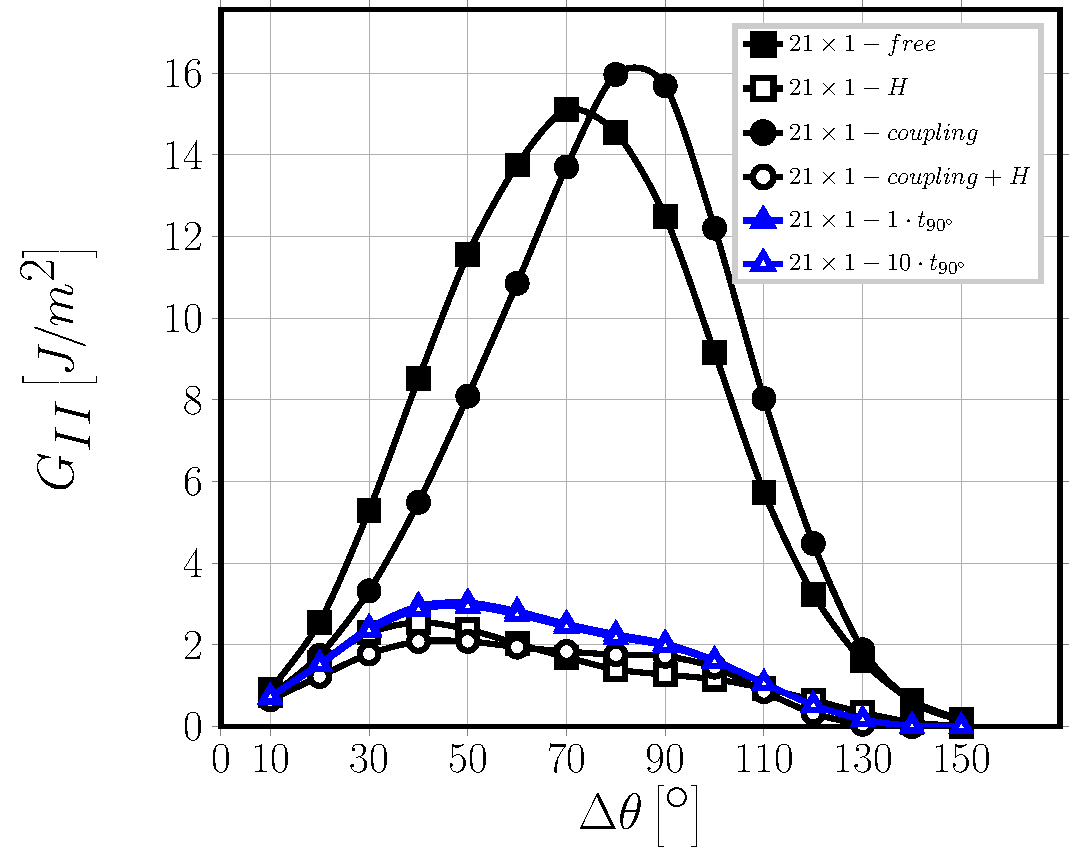
\includegraphics[height=0.375\textheight]{paperC/nx1-1-vf60-GII.pdf}
\caption{Effect of the presence of the $0^{\circ}$ layer on Mode II ERR of non-interactive debonds: models $21\times 1-free$, $21\times 1-H$, $21\times 1-coupling$, $21\times 1-coupling+H$, $21\times 1-1\cdot t_{90^{\circ}}$ and $21\times 1-10\cdot t_{90^{\circ}}$. $V_{f}=60\%$, $\bar{\varepsilon}_{x}=1\%$.}\label{paperC:fig:debonddebondGII}
\end{figure}

In agreement with the introductory considerations of this section and the results in~\cite{DiStasio2019}, it is possible to observe in Figures~\ref{paperC:fig:debonddebondGI} and~\ref{paperC:fig:debonddebondGII} that $21\times 1-free$ and $21\times 1-coupling$ (in which the horizontal displacement $u_{x}$ is left uncostrained on the upper boundary) show both the highest values of Mode I and Mode II ERR as well as the maximum increase with respect to the interactive case ($1\times 1-free$ and $1\times 1-coupling$). When the H-condition is applied to the upper boundary, thus constraining the magnitude of the strain magnification effect, both the magnitude of Mode I and Mode II ERR as well as their relative increase with respect to the interactive case are significantly reduced. $21\times 1-coupling+H$ represents, when considering both Mode I and Mode II ERR, the best approximation to the results of $21\times 1-m\cdot t_{90^{\circ}}$. The mechanisms at play are the same as in Sec.~\ref{paperC:subsec:thickness}: by keeping the $0^{\circ}/90^{\circ}$ interface straight (coupling condition), the $0^{\circ}$ layer favors an increase in $G_{I}$ and decrease in $G_{II}$ for small debonds and an increase in $G_{II}$ for large debonds; by applying a uniform $x$-strain on the $90^{\circ}$ layer boundary (H-condition), the $0^{\circ}$ layer promotes a more uniform $x$-strain in the $90^{\circ}$ layer and acts against the strain magnification effect, reducing debond ERR. Results in Fig.~\ref{paperC:fig:debonddebondGI} and Fig.~\ref{paperC:fig:debonddebondGII} show that the latter effect (H-condition) is dominant. It seems reasonable to conclude that debond growth is favored (i.e. debond ERR is higher) in the presence of strain or stress concentrations (as for example in the presence of a free surface or only coupling conditions on the vertical displacement), while more uniform strain and stress fields as those created by the proximity of the $0^{\circ}/90^{\circ}$ interface reduce both Mode I and Mode II ERR and thus tend to prevent debond growth.

\subsection{Effect of the presence of fiber rows with no damage on the debond-$0^{\circ}/90^{\circ}$ interface interaction}

After having investigated the effect of the proximity of the $0^{\circ}/90^{\circ}$ interface and of the thickness of the $0^{\circ}$ layer on debond ERR for different cases of debond-debond interaction in the same fiber row, we address in this section the effect of the presence of fiber rows with only fully bonded fibers between debonds and the $0^{\circ}/90^{\circ}$ interface. In other words, we are separating the debond from the $0^{\circ}/90^{\circ}$ interface by inserting rows of fully bonded fibers in between. We consider only the case $m=1$, i.e. $t_{0^{\circ}}=t_{90^{\circ}}$, given that increasing the $0^{\circ}$ layer thickness does not result in any remarkable effect on ERR as shown in Sec.~\ref{paperC:subsec:thickness} and Sec.~\ref{paperC:subsec:debonddebondinter}. Following the same philosophy of Sec.~\ref{paperC:subsec:thickness} and Sec.~\ref{paperC:subsec:debonddebondinter}, we analyze the effect of the presence of fiber rows with no damage on debond ERR: first, when the central fiber row possesses only partially debonded fibers, which represents the most severe damage state for these RUCs and the solution for interactive debonds (models $1\times k-1\cdot t_{90^{\circ}}$ in Figures~\ref{paperC:fig:1kGI} and~\ref{paperC:fig:1kGII}); second, the case of debonds separated by $n-1$ fully bonded fibers in the central fiber row, which corresponds to the least severe state of damage and to the solution for non-interactive debonds (models $21\times k-1\cdot t_{90^{\circ}}$ in Figures~\ref{paperC:fig:nkGI} and~\ref{paperC:fig:nkGII}).\\%Figures~\ref{paperC:fig:1kGI} and~\ref{paperC:fig:1kGII} thus show the effect on ERR of the presence of the $0^{\circ}$ ply in the case of non-interacting debonds (no strain magnification or crack shielding). If the distance between the $0^{\circ}/90^{\circ}$ interface and the debond is at least one fully bonded fiber, the presence of the $0^{\circ}$ ply does not influence debond ERR and no measurable difference can be observed between models $1\times k-free$ and $1\times k-1\cdot t_{90^{\circ}}$ for $k\geq1$.

\begin{figure}[!htb]
\centering
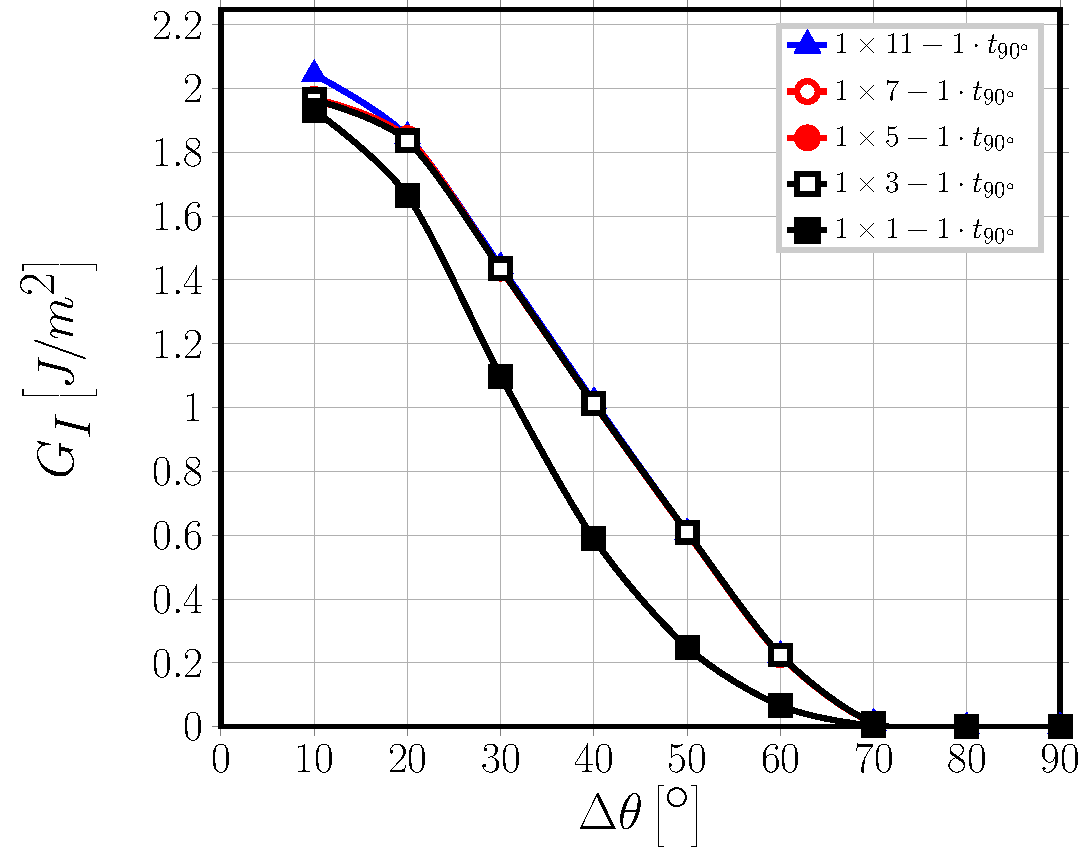
\includegraphics[height=0.375\textheight]{paperC/1xk-1-vf60-GI.pdf}
\caption{Effect of the presence of undamaged fiber rows in the $90^{\circ}$ layer on debond-$0^{\circ}/90^{\circ}$ interface interaction for Mode I ERR: models $1\times k-1\cdot t_{90^{\circ}}$. $V_{f}=60\%$, $\bar{\varepsilon}_{x}=1\%$.}\label{paperC:fig:1kGI}
\end{figure}

Observation of Fig.~\ref{paperC:fig:1kGI}, Fig.~\ref{paperC:fig:1kGII}, Fig.~\ref{paperC:fig:nkGI} and Fig.~\ref{paperC:fig:nkGII} reveals that no difference can be seen in Mode I and Mode II ERR by increasing the number $k$ of rows with undamaged fibers when $k\geq3$, which means that debond ERR does not change once at least $1$ row of undamaged fibers is present between the debond and the $0^{\circ}/90^{\circ}$ interface. A significant change is visible only when $k=1$, which means that no row of undamaged fibers is present between the debond and the $0^{\circ}/90^{\circ}$ interface. This change, from $k\geq3$ to $k=1$, corresponds in particular to a reduction of both $G_{I}$ and $G_{II}$.

\begin{figure}[!htb]
\centering
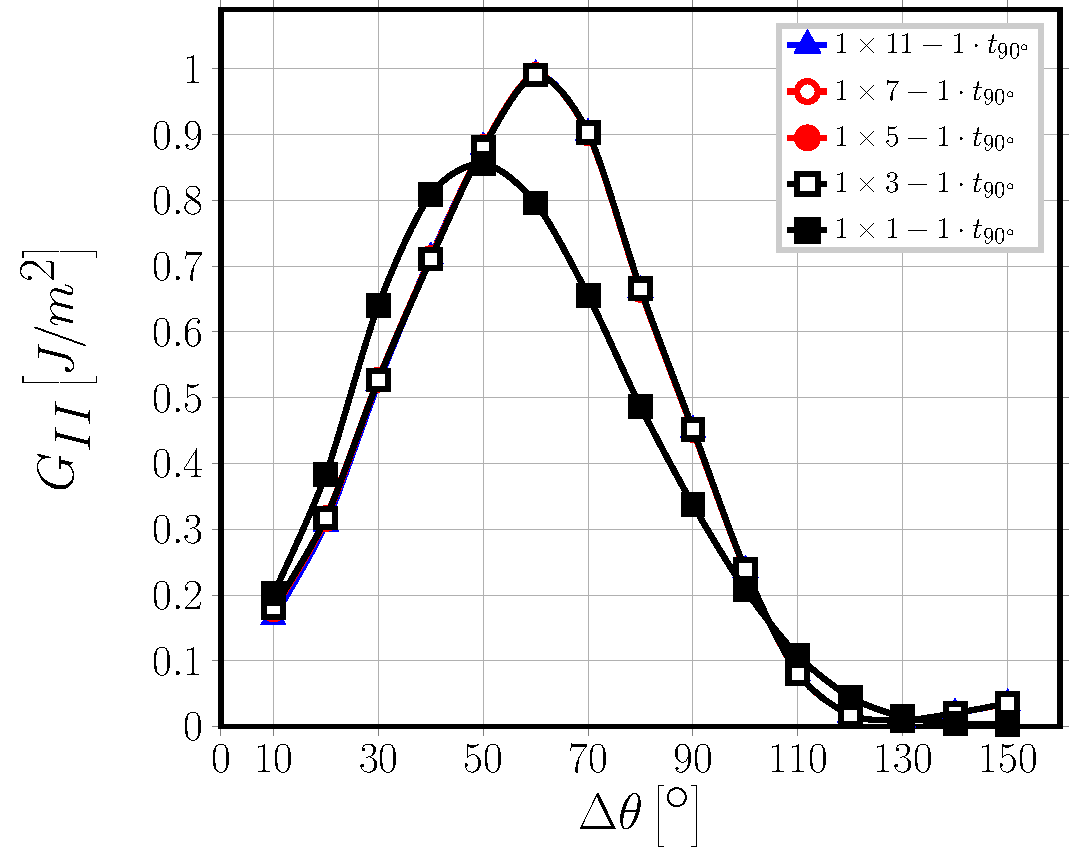
\includegraphics[height=0.375\textheight]{paperC/1xk-1-vf60-GII.pdf}
\caption{Effect of the presence of undamaged fiber rows in the $90^{\circ}$ layer on debond-$0^{\circ}/90^{\circ}$ interface interaction for Mode II ERR: models $1\times k-1\cdot t_{90^{\circ}}$. $V_{f}=60\%$, $\bar{\varepsilon}_{x}=1\%$.}\label{paperC:fig:1kGII}
\end{figure}

The results of Figures~\ref{paperC:fig:1kGI}, \ref{paperC:fig:1kGII}, \ref{paperC:fig:nkGI} and~\ref{paperC:fig:nkGII} imply that the mechanisms of debond-$0^{\circ}/90^{\circ}$ interface interaction described in Sec.~\ref{paperC:subsec:thickness} and Sec.~\ref{paperC:subsec:debonddebondinter} are actually very localized and that debond ERR is affected by the presence of the $0^{\circ}/90^{\circ}$ interface only when no fully bonded fiber is placed in between. Given that the number $k$ of fibers in the RUC vertical direction corresponds to the thickness of the $90^{\circ}$ ply measured in terms of number of fiber rows present through its thickness, the results presented here point to another conclusion: the ply-thickness effect does not seem to apply to debond growth, unless an \textit{ultra-thin} ply constituted by only one fiber row ($k=1$) is considered.\\

\begin{figure}[!htb]
\centering
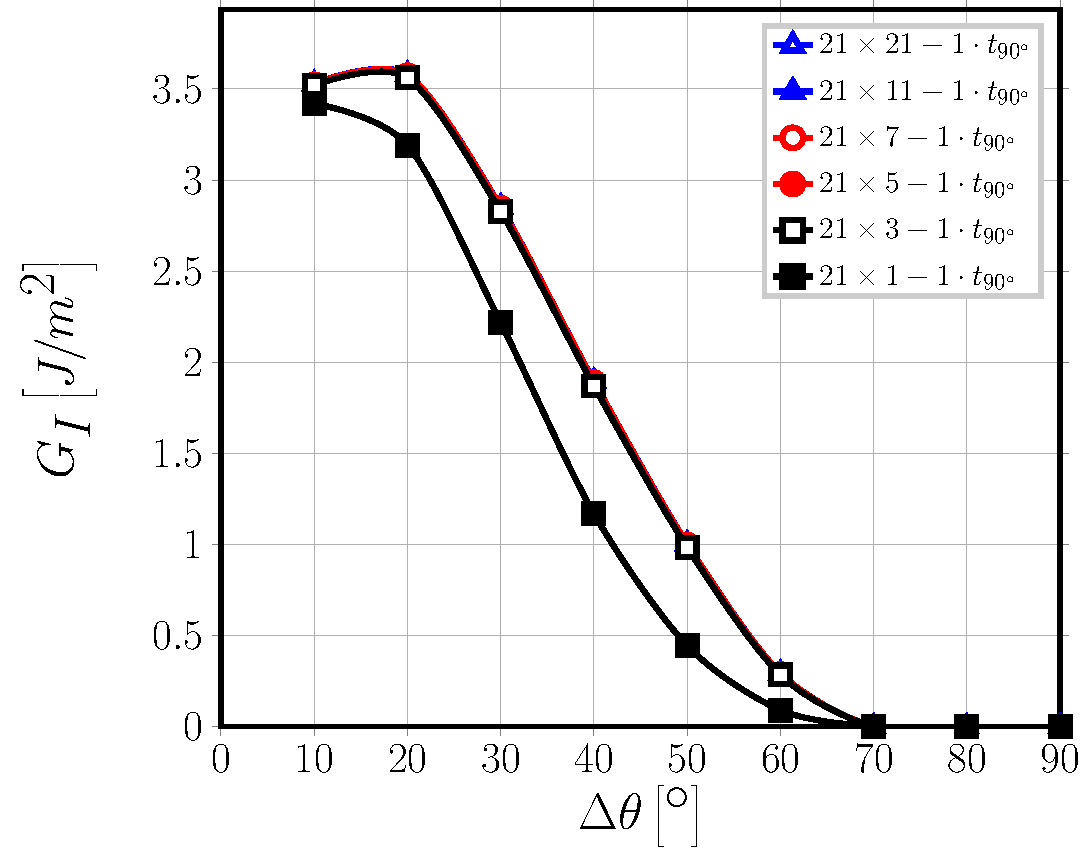
\includegraphics[height=0.375\textheight]{paperC/nxk-1-vf60-GI.pdf}
\caption{Effect of the presence of undamaged fiber rows in the $90^{\circ}$ layer on debond-$0^{\circ}/90^{\circ}$ interface interaction for Mode I ERR: models $n\times k-1\cdot t_{90^{\circ}}$. $V_{f}=60\%$, $\bar{\varepsilon}_{x}=1\%$.}\label{paperC:fig:nkGI}
\end{figure}

Analogous results can be found in~\cite{Velasco2018, Paris2018}, where the authors investigate the ply-thickness effect on debond growth in cross-ply laminates using: first, a single centrally-placed partially debonded fiber with surrounding matrix corresponding to $V_{f}=55\%$, embedded from all sides in a homogenized $90^{\circ}$ ply bounded by homogenized $0^{\circ}$ layers; second, one partially debonded fiber placed in the center and a second partially debonded fiber placed at an angle $\theta_{2}$ with respect to the horizontal direction with surrounding matrix corresponding to $V_{f}=55\%$, embedded from all sides in a homogenized $90^{\circ}$ ply bounded by homogenized $0^{\circ}$ layers. The thickness of the $0^{\circ}$ layer is chosen as reference and a $\left[0^{\circ}_{p},90^{\circ}_{r\cdot p}\right]_{S}$ laminate is considered. Carbon-epoxy and glass-epoxy systems are both studied. The thickness of the $90^{\circ}$ ply, $t_{90^{\circ}}=r\cdot t_{0^{\circ}}$, varies from $r=3$ (thick $90^{\circ}$ ply, $>100$ fiber diameters) to $r=0.1$ (thin $90^{\circ}$ ply, $\sim4-5$ fiber diameters). No measurable ply-thickness effect was observed. Experimental support to the claim that the ply-thickness effect has no influence on debond growth can be also found in the literature, in~\cite{Saito2012}. The authors conducted \emph{in-situ} observations of edge micro-cracks with an optical microscope on $\left[0^{\circ}_{2},90^{\circ}_{n},0^{\circ}_{2}\right]$ carbon fiber-epoxy laminates with $n=1,2,4$, corresponding to a $90^{\circ}$ ply thickness of respectively $40\ [\mu m]$ ($\sim 6-8$ fiber diameters), $80\ [\mu m]$  ($\sim 12-16$ fiber diameters) and $160\ [\mu m]$  ($\sim 24-32$ fiber diameters). For $n=1$, i.e. the case of a very thin $90^{\circ}$ ply, isolated debonds appear at a lower value of the applied strain than in thicker plies (at $0.4\%$ vs $0.7\%$) while growth and coalescence of debonds is suppressed and no transverse crack can be observed even at a strain of $1.5\%$. The ply-thickness effect was thus observed in~\cite{Saito2012} for transverse cracks, i.e. coalescence of debonds was delayed to higher strains and even suppressed, but not for debond growth. The analysis presented in this article brings new arguments to the claim that the ply-thickness effect does not influence the growth of debonds.

\begin{figure}[!htb]
\centering
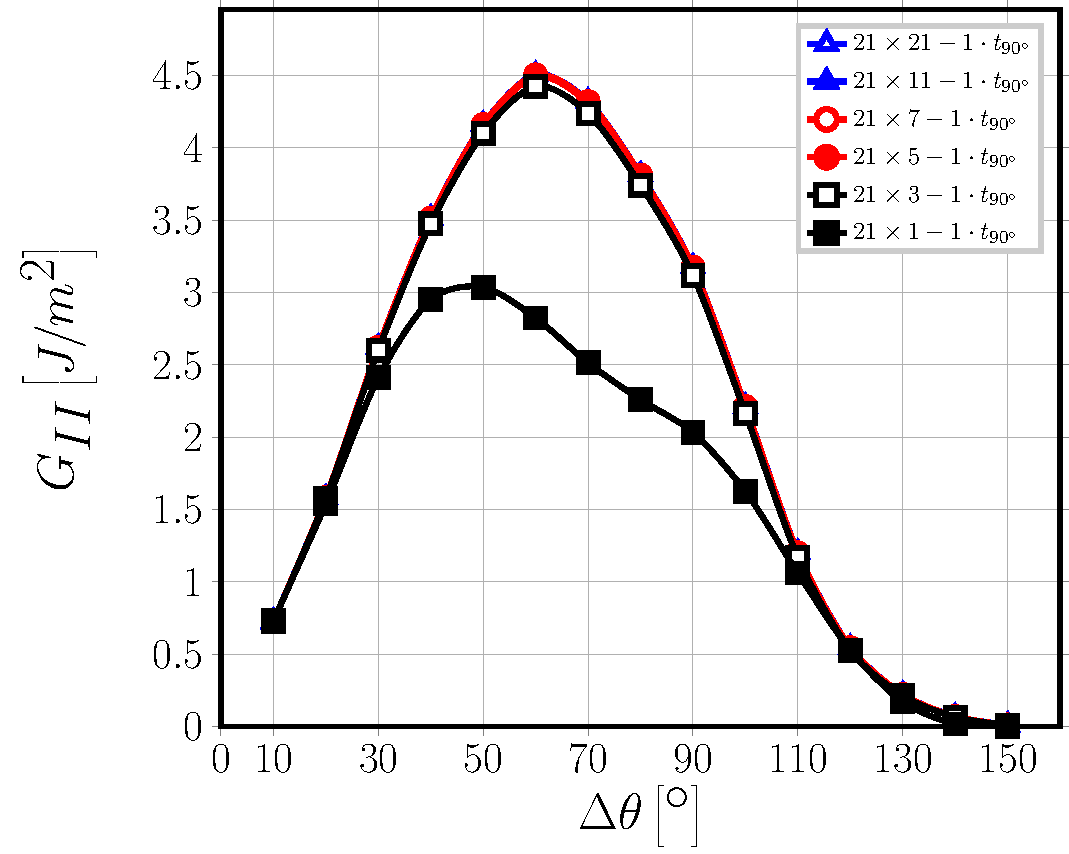
\includegraphics[height=0.375\textheight]{paperC/nxk-1-vf60-GII.pdf}
\caption{Effect of the presence of undamaged fiber rows in the $90^{\circ}$ layer on debond-$0^{\circ}/90^{\circ}$ interface interaction for Mode II ERR: models $n\times k-1\cdot t_{90^{\circ}}$. $V_{f}=60\%$, $\bar{\varepsilon}_{x}=1\%$.}\label{paperC:fig:nkGII}
\end{figure}

%%%%%%%%%%%%%%%%%%%%%%%%%%%%%%%%%%%%%%%%%%%%%%%%%%%%%%%%%%%%%%%%%%%
% 4. CONCLUSIONS AND OUTLOOK
%%%%%%%%%%%%%%%%%%%%%%%%%%%%%%%%%%%%%%%%%%%%%%%%%%%%%%%%%%%%%%%%%%%

\section{Conclusions}

Different models of Repeating Unit Cell, representing different cross-ply laminates, have been studied in order to investigate the effect of the presence of the $0^{\circ}$ layer and of its thickness on debond Energy Release Rate for interactive and non-interactive debonds. A particular damage state is studied, in which only the central row of fibers of the $90^{\circ}$ ply possesses debonds. The thickness of the $90^{\circ}$ ply is measured in terms of the number of fiber rows in the layer; the $0^{\circ}$ layer is on the other hand modelled as a homogenized material, the thickness of which is a multiple of the $90^{\circ}$ ply thickness. In order to investigate the mechanisms of the debond-$0^{\circ}/90^{\circ}$ interface interaction, Mode I and Mode II ERR of cross-ply RUCs are compared with those of RUCs with equivalent boundary conditions on the upper boundary: free surface; coupling conditions on the vertical displacements; an applied linear distribution of the horizontal displacement; coupling conditions on the vertical displacements superimposed to an applied linear distribution of the horizontal displacement (this last combination represents the most extreme effect of the $0^{\circ}$ layer on debond growth). It has been found that:
\begin{itemize}
\item by forcing the $0^{\circ}/90^{\circ}$ interface to remain approximately straight and controlling the uniformity of the horizontal displacements in the composite (and thus in the $90^{\circ}$ ply), the presence of the $0^{\circ}$ layer causes more homogeneous local (i.e. in the debond neighborhood) strains, reducing the ERR at the debond crack tip;
\item when increasing the thickness of the $0^{\circ}$ layer, the effect of the presence of the $0^{\circ}$ layer on debond ERR remains the same as in the case $t_{0^{\circ}}=t_{90^{\circ}}$;
%\item no difference in ERR is seen when one or more rows of fibers with no damage are present between the debond and the $0^{\circ}/90^{\circ}$ interface, a change is observed only no row of undamaged fibers is present between the debond and the $0^{\circ}/90^{\circ}$ interface;
\item no effect of the $90^{\circ}$ layer thickness, measured in terms of number of fiber rows, is observed; a reduction in ERR takes place only when the thickness is reduced to only one fiber row.
\end{itemize}
The results reported in this article strengthen the claim that the ply-thickness effect does not influence the growth of individual debonds, as previously suggested in the literature~\cite{Saito2012,Herraez2015,Velasco2018, Paris2018}.

%%%%%%%%%%%%%%%%%%%%%%%%%%%%%%%%%%%%%%%%%%%%%%%%%%%%%%%%%%%%%%%%%%%
% ACKNOWLEDGEMENTS
%%%%%%%%%%%%%%%%%%%%%%%%%%%%%%%%%%%%%%%%%%%%%%%%%%%%%%%%%%%%%%%%%%%

\section*{Acknowledgements}

Luca Di Stasio gratefully acknowledges the support of the European School of Materials (EUSMAT) through the DocMASE Doctoral Programme and the European Commission through the Erasmus Mundus Programme.


\section*{References}
\addcontentsline{toc}{section}{References}
\printbibliography[heading=none]
